\documentclass[12pt]{article}

\usepackage{amsmath}
\usepackage{amsthm}
\usepackage{amssymb}
\usepackage{mathtools}
\usepackage{latexsym}
\usepackage{cancel}
\usepackage{tikz}

\usepackage{fancyhdr}

\usepackage{float}
\usepackage{graphicx}
\usepackage{pagecolor}
\usepackage{xcolor}

\usepackage{inputenc}
\usepackage[T1]{fontenc}
\usepackage[default]{lato}
\usepackage{contour}
\usepackage{ulem}


\usepackage[
top=2.50cm,
bottom=2.50cm,
left=2cm,
right=2cm,
marginparsep=0pt,
marginparwidth=0pt]{geometry}

\parindent 0in
\parskip 12pt

\definecolor{Ivory Paper}{HTML}{F7F0DF}

\pagecolor{Ivory Paper}

\newcommand{\floor}[1]{\left\lfloor #1 \right\rfloor}
\newcommand{\ceil}[1]{\left\lceil #1 \right\rceil}
\newcommand{\round}[1]{\left\lfloor #1 \right\rceil}
\newcommand{\abs}[1]{\left\lvert #1 \right\rvert}
\newcommand{\sqref}[1]{[\ref{#1}]}

\DeclareRobustCommand{\ul}[1]{%
	\uline{\phantom{#1}}%
	\llap{\contour{white}{#1}}%
}

\renewcommand{\ULdepth}{1.8pt}
\contourlength{0.8pt}

\theoremstyle{plain}
\newtheorem{thm}{Theorem}
\newtheorem{cor}{Corollary}
\newtheorem{lma}{Lemma}
\newtheorem{prop}{Proposition}
\newtheorem{conj}{Conjecture}
\newtheorem{defn}{Definition}

\setlength{\headheight}{15pt}
\pagestyle{fancy}
\renewcommand{\headrulewidth}{0pt}
\lhead{J. Scerri}
\chead{Personal Research}
\rhead{\thepage}

% TITLE

\title{Graph Theory\\
\vspace{0.75em}\textbf{Personal Research}}

\date{\today}

\author {{\textbf{Juan Scerri}}\\
B.Sc. (Hons)(Melit.) Computing Science and Mathematics (Second Year)}

\begin{document}

\maketitle % Print the title page

\thispagestyle{empty} % Suppress headers and footers on the title page

\begin{conj}[Erd\H os–Gy\` arf\` as Conjecture]

Every simple graph $G$ with minimum degree $3$ contains a simple
cycle whose length is a power of two.

\end{conj}

At first glance there does not seem any clear way to approach
the problem. So instead we will define a weaker version of the
conjecture. Hopefully, the machinery developed for solving the
weaker conjecture will prove to be useful when tackling the full
conjecture.

\begin{conj}

Every simple graph $G$ with minimum degree $3$ contains a simple
cycle whose length is even.

\end{conj}

We will try to approach this by assuming that the all cycles are
of odd length. Now we need to look at the most general way
cycles of odd length can interact with each other.

\begin{defn}
Let $C$ be a cycle. $C$ is said to be a $k$--mod--cycle if and
only if the length of $C$ is divisible by $k$.
\end{defn}

\begin{defn}
A $2$--mod--cycle is said to be an even cycle. And a
non--$2$--mod--cycle is a said to be an odd cycle. 
\end{defn}

\begin{prop}\label{edge-connected-cycles}
If $G$ and $H$ are two odd cycles connected by at least two
edges (let this graph be $F$), then $F$ contains an even cycle. 
\end{prop}

\begin{proof}
    Let $V(G) = \{g_1, g_2, \ldots, g_k\}$ and $V(H) = \{h_1,
    h_2, \ldots, h_l\}$ where $k$ and $l$ are odd numbers
    greater than $3$. Pick any two vertices in $V(G)$ say $g_a$
    and $g_b$ and pick any two vertices in $V(H)$ say $h_c$ and
    $h_d$ such that $h_c \not = h_d$. $h_c$ and $h_d$ cannot be
    equal because if they where and $g_a = g_b$, then we would
    have connected the cycles with only one unique edge but we
    want do do so with two distinct edges.

    Since, the length of $G$ is odd picking any two vertices
    (even the same vertex) will split the cycle into two, a
    segment having even length and a segment having odd length.
    Similarly, this will happen on $H$ as well. Starting from
    $h_c$, traverse the even path to $h_d$. Crossover, to $H$
    using the edge connected to $h_d$. Say this is connected to
    $g_b$. From $g_b$ traverse the even path to $g_a$. Then
    crossover again to $h_c$. This completes the cycle and the
    cycle is even since both paths have the same parity and we
    are adding $2$ because of the two crossovers.
\end{proof}

\begin{prop}
If $G$ and $H$ are two odd cycles and they share at least $2$ and at most \\ $\max\{V(G), V(H)\} - 1$ vertices (let
this graph be $F$), then $F$ contains an even cycle. 
\end{prop}

\begin{prop}
If $G$ and $H$ are two odd cycles connected by at least two
paths of length greater than 1 (let this graph be $F$), then $F$
contains an even cycle. 
\end{prop}

TODO: The above proof should be almost as the proof for
proposition simple to prove as the proof for proposition
\ref{edge-connected-cycles}. The basic idea is as follows look
at the graph $F$ if it has two paths of the same parity
connecting $G$ and $H$ this is reduced to the case for
proposition \ref{edge-connected-cycles} since adding two lengths
of same parity and another two lengths of same parity will
result in a final length of even parity. The only difficulty is
considering the case when one cannot pick two paths which have
identical parity. In that case one is forced to traverse the
segment of one of the cycles which has opposite parity to the
segment walk on the other. Hence giving us two length which are
of same parity and another two lengths which are of same parity.
Hence, the total is also guaranteed to be even.

So it is true for odd cycles which are connected by at least two
paths. What about shared vertices. This is a more complicated
endeavour. Additionally, it will also be more complicated to
show this for when a mixture of the two types is present. But
let us suppose for second that we have shown that said
statements are true. Using this knowledge we can try to show
that our weak conjecture is true.

So suppose that we have a connected minimum degree 3 graph and
that all cycles is said graph are odd. Now what we want to show
is that any 
about our contradiction 

TODO: Add exposition as to why I arrived at this point.

\begin{figure}[H]
\centering
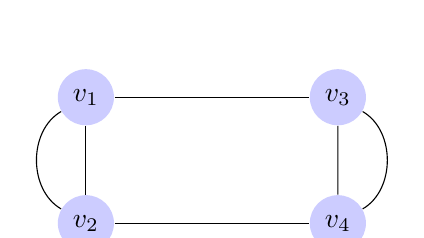
\begin{tikzpicture}
  [scale=.8,auto=center,every node/.style={circle,fill=blue!20}]

  \node (v1) at (0,2) {$v_1$};
  \node (v2) at (0,0) {$v_2$};
  \node (v3) at (4,2) {$v_3$};
  \node (v4) at (4,0) {$v_4$};

  \foreach \from/\to in {v1/v2,v3/v4,v1/v3,v2/v4}
    \draw (\from) -- (\to);

  \draw (v1) edge [bend right = 6em] (v2);
  \draw (v3) edge [bend left = 6em] (v4);
\end{tikzpicture}
\caption{Smallest non--trivial case}
\end{figure}

So all the different paths in the above configuration are the
following:

\begin{enumerate}
\item $v_1 v_2 v_4 v_3$
\item $v_1 v_2 v_4 v_3$
\item $v_1 v_2 v_4 v_3$
\item $v_1 v_2 v_4 v_4$
\end{enumerate}

TODO: Introduce labels for this case only because technically
this is a multigraph. However, it is still a valid case for
analysis in our case.

\begin{figure}[H]
\centering
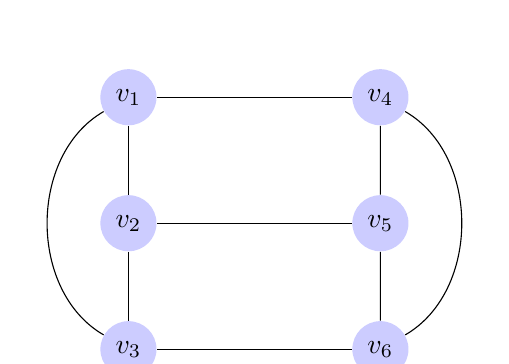
\begin{tikzpicture}
  [scale=.8,auto=center,every node/.style={circle,fill=blue!20}]

  \node (v1) at (0,4) {$v_1$};
  \node (v2) at (0,2) {$v_2$};
  \node (v3) at (0,0) {$v_3$};
  \node (v4) at (4,4) {$v_4$};
  \node (v5) at (4,2) {$v_5$};
  \node (v6) at (4,0) {$v_6$};

  \foreach \from/\to in
  {v1/v2,v2/v3,v4/v5,v5/v6,v1/v4,v2/v5,v3/v6}
    \draw (\from) -- (\to);

  \draw (v1) edge [bend right = 6em] (v3);
  \draw (v4) edge [bend left = 6em] (v6);
\end{tikzpicture}
\caption{The 3 case}
\end{figure}

Again we will manually count all of the unique cycles. (From 3
onwards we do not need to worry about the ambiguity of our
notation since these are not multigraphs).

\begin{enumerate}
\item $v_1 v_2 v_5 v_4 v_1$
\item $v_2 v_3 v_6 v_5 v_2$
\item $v_1 v_4 v_6 v_3 v_1$
\item $v_1 v_2 v_5 v_6 v_4 v_2$
\item $v_1 v_2 v_3 v_6 v_4 v_1$
\item $v_2 v_3 v_1 v_4 v_5 v_2$
\item $v_2 v_3 v_1 v_4 v_5 v_6 v_2$
\item $v_1 v_2 v_3 v_6 v_5 v_4 v_1$
\item $v_4 v_5 v_2 v_1 v_3 v_6 v_4$
\end{enumerate}

Note: From what I recall you can only have an even number of 
crossings across the bridges formed. An odd number of crossings
is impossible. Since you would connect back to something which
you already visited which is not actually your returning
node.

\begin{figure}[H]
\centering
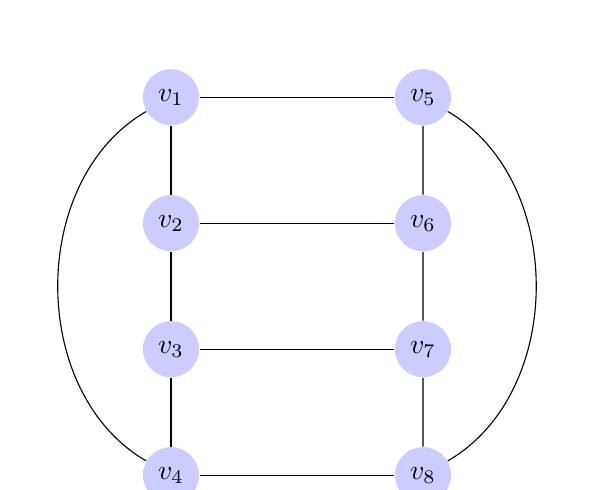
\begin{tikzpicture}
  [scale=.8,auto=center,every node/.style={circle,fill=blue!20}]

  \node (v1) at (0,6) {$v_1$};
  \node (v2) at (0,4) {$v_2$};
  \node (v3) at (0,2) {$v_3$};
  \node (v4) at (0,0) {$v_4$};
  \node (v5) at (4,6) {$v_5$};
  \node (v6) at (4,4) {$v_6$};
  \node (v7) at (4,2) {$v_7$};
  \node (v8) at (4,0) {$v_8$};

  \foreach \from/\to in
  {v1/v2,v2/v3,v3/v4,v5/v6,v6/v7,v7/v8,v1/v5,v2/v6,v3/v7,v4/v8}
    \draw (\from) -- (\to);

  \draw (v1) edge [bend right = 6em] (v4);
  \draw (v5) edge [bend left = 6em] (v8);
\end{tikzpicture}
\end{figure}

\end{document}

